\section{Structure from Motion}
\label{sfm}

The last part of the lab assignment discusses the final parts of the Structure from Motion (SFM) algorithm. In particular, using the output of the assignment's $2^{nd}$ part, we derive the motion and shape matrix of a given set of points.  

\subsection{Implementation Details}
As mentioned above, the data used by this part of the algorithm is an $m\times n$ matrix, where $m$ is the total number of frames, and $n$ is the total number of feature points extracted by the previous step of SFM. 
Given this "Point View" matrix, we gather feature points that persist through a sufficient number of frames, and construct a new $A: 2m\times n'$ matrix, where each row represents a 2D coordinate of each of $n'$ feature points. Note that this matrix is dense enough to adequately describe 3D structure given 2D feature points.

After obtaining matrix $A$, 3D coordinates must be calculated for each feature point, with respect to every frame. In order to achieve that, we need to normalize the 2D coordinates in $A$. For each row of the $A$ matrix, we calculate the centroid (the average coordinate over all feature points) which then we subtract from every point coordinate in the same row. By doing this, we relate every feature point to a 3D position in the resulting 3D structure.

Following normalization, SVD is applied to the (normalized) $A$ matrix to obtain the motion \& shape matrices:  
$D = U\times W\times V^T$

We need to reduce the rank of the resulting matrices to 3, in order to obtain 3D coordinates, so we use the 3 first columns of $U$, the 3 first rows of $V^T$ and the top-left $3\times 3$ matrix of $W$ to obtain $U_3, W_3,$ and $V^T_3$. Lastly, the matrix \& shape functions are given by: $M = U_3W^{\frac{1}{2}}_3$, $S = W_3^{\frac{1}{2}}V^T_3$

\subsection{Dealing with affine ambiguity}
The process described before, implies a decomposition that is subject to affine transformation\cite{amb}. Taking that into account, we further factorize matrices $M\rightarrow \hat{M}$ \& $S\rightarrow \hat{S}$ according to Morita and Kanade (1997)\cite{amb}. In more detail, we calculate matrix $A^{-1}$ and $A$ where $A$ represents an affine transform that transforms $\hat{M}$ into $M$ and $A^{-1}$ transforms $\hat{S}$ into $S$. Applying these matrix manipulations erases the affine ambiguity, under the assumption that image axes must be perpendicular\cite{amb}.

Looking at figures ~\ref{fig:icp4-11-Amb} and ~\ref{fig:icp4-11}, we can se that the latter has a slightly better structure, as far as the density and the distance between feature points is concerned. 

\subsection{Frame sampling}
We have observed that many feature points are detected at non-informative positions, implying a noise factor in our SFM implementation. In order to reduce the noise, while also increasing the speed of the algorithm, we sampled though the frame set, by skipping 1, 2, 4, 5 or 8 frames. 


\subsection{Results}

Below, we present the results obtained by the SFM implementation. 

\begin{figure}[ht!]
  \centering
    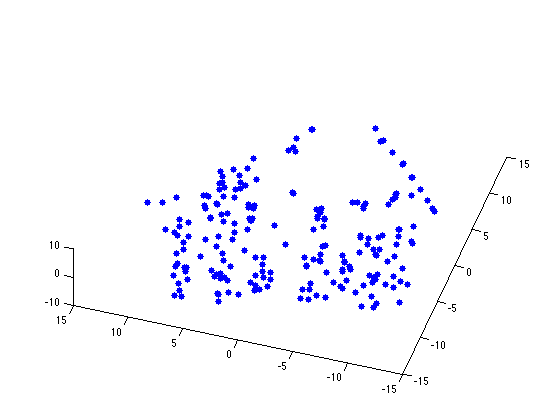
\includegraphics[width=0.49\textwidth]{figures/icp1-46-Amb.png}
    \caption{3D structure of the house frameset, sampling all frames, without affine ambiguity correction.}
    \label{fig:icp1-46-Amb}
\end{figure}

\begin{figure}[ht!]
  \centering
    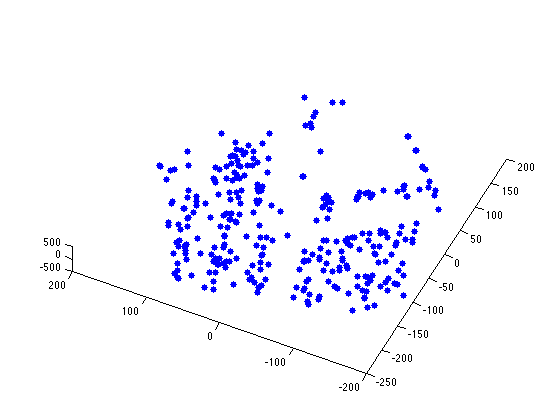
\includegraphics[width=0.49\textwidth]{figures/icp2-22.png}
    \caption{3D structure of the house frameset, sampling every 2 frames, with affine ambiguity correction.}
    \label{fig:icp2-22}
\end{figure}


\begin{figure}[ht!]
  \centering
    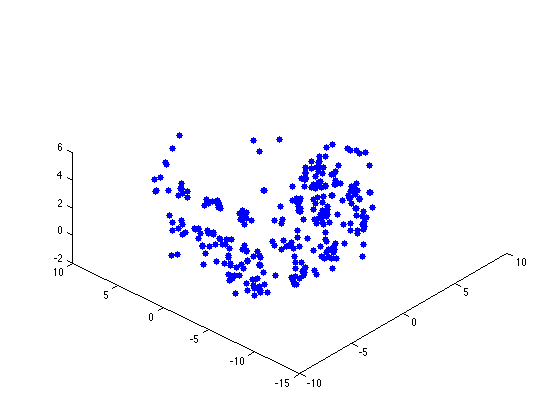
\includegraphics[width=0.49\textwidth]{figures/icp4-11-Amb.png}
    \caption{3D structure of the house frameset, sampling every 4 frames, without affine ambiguity correction.}
    \label{fig:icp4-11-Amb}
\end{figure}

\begin{figure}[ht!]
  \centering
    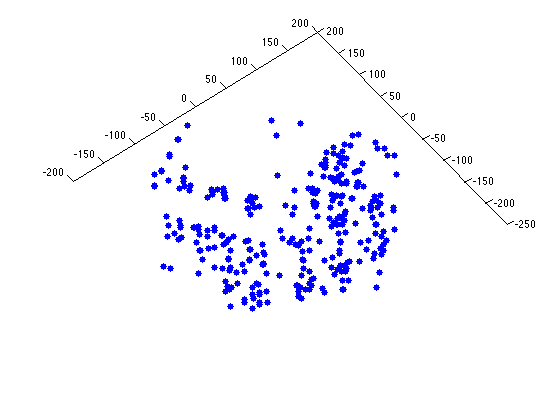
\includegraphics[width=0.49\textwidth]{figures/icp4-11.png}
    \caption{3D structure of the house frameset, sampling every 4 frames, with affine ambiguity correction.}
    \label{fig:icp4-11}
\end{figure}

\begin{figure}[ht!]
  \centering
    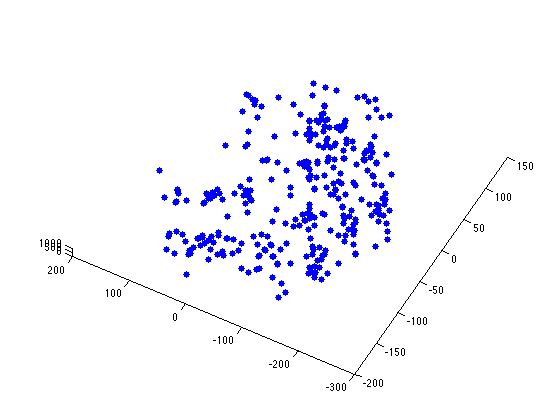
\includegraphics[width=0.49\textwidth]{figures/icp5-8.png}
    \caption{3D structure of the house frameset, sampling every 5 frames, with affine ambiguity correction.}
    \label{fig:icp5-8}
\end{figure}

\begin{figure}[ht!]
  \centering
    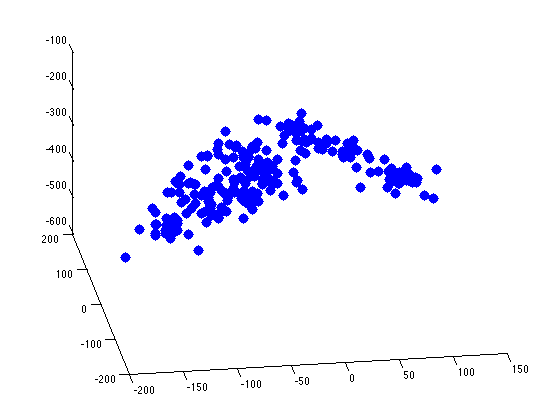
\includegraphics[width=0.49\textwidth]{figures/icp8-5.png}
    \caption{3D structure of the house frameset, sampling every 8 frames, with affine ambiguity correction.}
    \label{fig:icp8-5}
\end{figure}



\subsection{Discussion}
This last step of the SFM algorithm gave us the opportunity to observe the results in practice. Given a set of frames, we used SFM to construct a 3D model of the object presented. 

However, while experimenting with two different sets of frames (House \& Teddybear), we discovered that the teddybear frameset is not capable of producing an efficient 3D model, while the house frameset does. An explanation to why this happens lies not in the actual implementation of the algorithm, but the dataset itself. It is a fact that the teddybear frameset contains a 360 degree y-axis rotation of the object, resulting in significantly less feature points being persistent through a large number of frames. 
On the other hand, the house frameset does not contain such steep change in point of view, but only a slight z-axis rotation. As a result, the number of feature points detected in all frames is higher, thus, the 3D model reconstructed by SFM looks more realistic.

Furthermore, regarding the frame sampling we introduced, we can observe an improvement from figure ~\ref{fig:icp1-46-Amb} to figure ~\ref{fig:icp4-11-Amb}, in terms of how realistic the structure looks. We can see that many new feature points are introduced, while in figure ~\ref{fig:icp4-11}, almost no noisy points are present.

Despite the improvement achieved, we can observe in figures ~\ref{fig:icp5-8} and ~\ref{fig:icp8-5} that sparse sampling can lead to undesired results. The structure of the house is inconsistent, especially in figure ~\ref{fig:icp8-5} where only feature points on the house roof are detected in all sampled frames. 

\section{Printable 3D Model}

\subsection{PCL (C++)}
In order to build a printable 3D model given a point cloud, we used the Point Cloud Library (PCL)\cite{pcl}. PCL has built-in functions in order to read and visualize a 3D point cloud using triangulation. 

\subsection{MyCrust (MATLAB)}
In order to visualize a 3D point cloud in MATLAB, we used the "myCrust.m" toolbox\cite{myc}. The functions it supplies construct a triangular mesh given a point cloud as input. In order to retrieve the data, we used the given readPcd() function, while we also used the MATLAB built-in function imfill() to create a watertight model. The latter function will "fill the holes" of every plane in the whole dataset. 

Snapshots of the visualization are presented in the section below.
\subsection{Results} 


\begin{figure}[ht!]
  \centering
    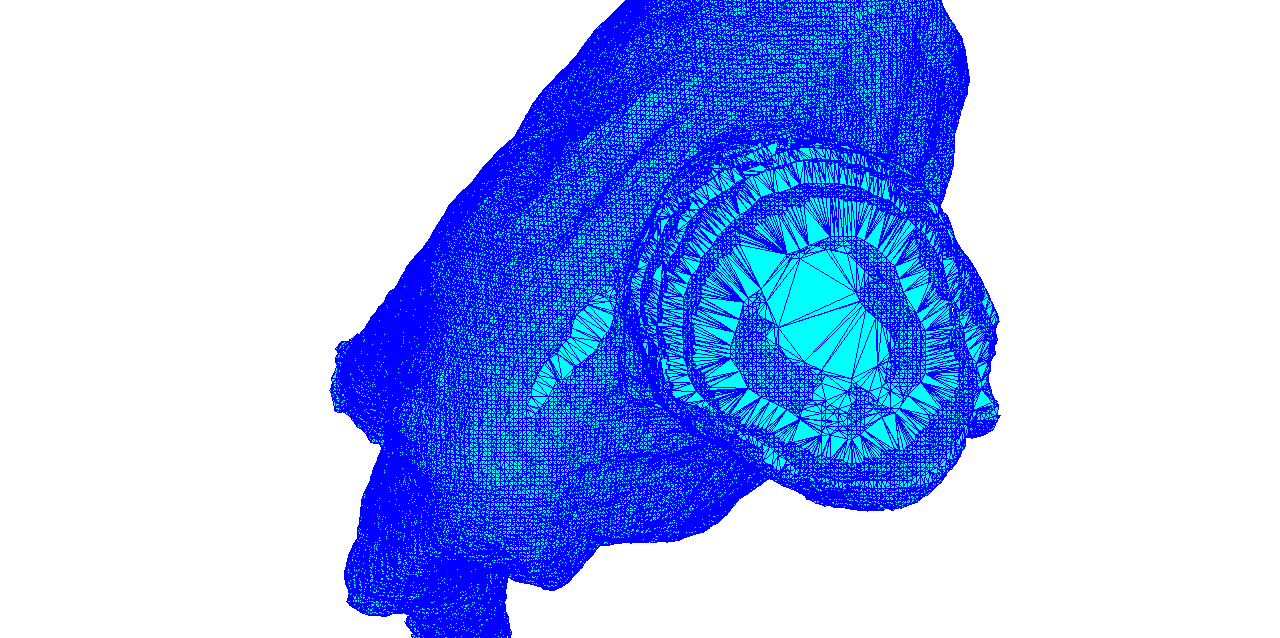
\includegraphics[width=0.49\textwidth]{figures/3dMesh_sundin_zoom_top.png}
    \caption{Printable triangular mesh, top view}
    \label{fig:sundin-top-zoom}
\end{figure}

\begin{figure}[ht!]
  \centering
    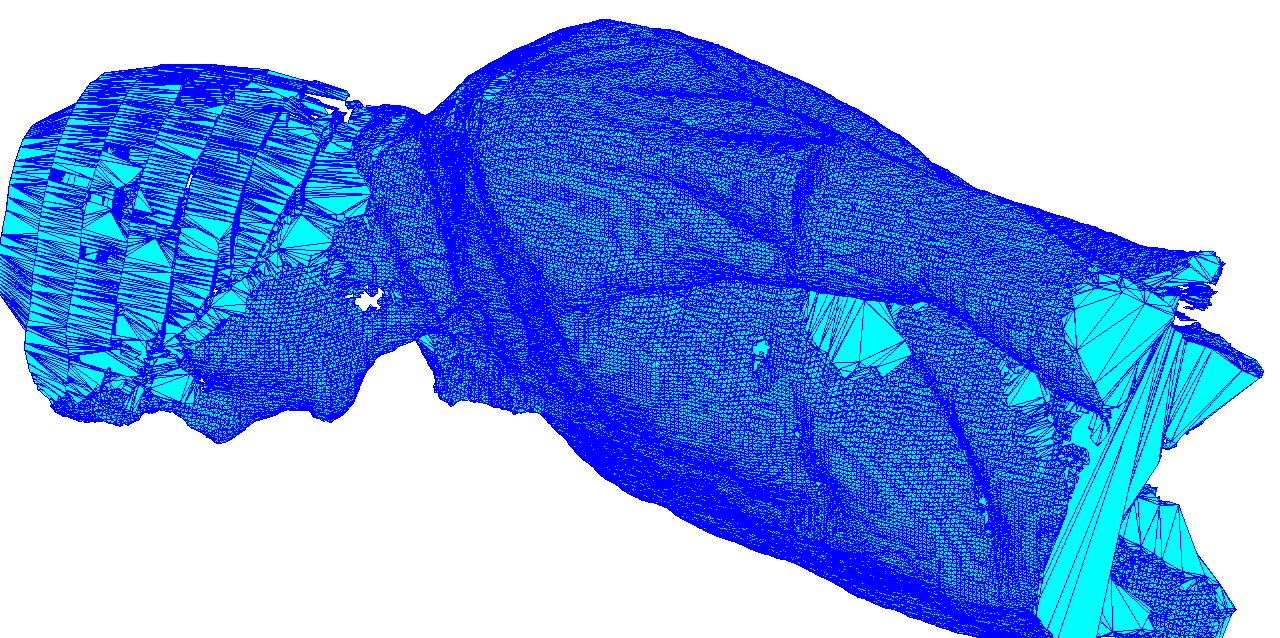
\includegraphics[width=0.49\textwidth]{figures/3dMesh_sundin_zoom_side.png}
    \caption{Printable triangular mesh, side view}
    \label{fig:sundin-top-zoom}
\end{figure}

\begin{figure}[ht!]
  \centering
    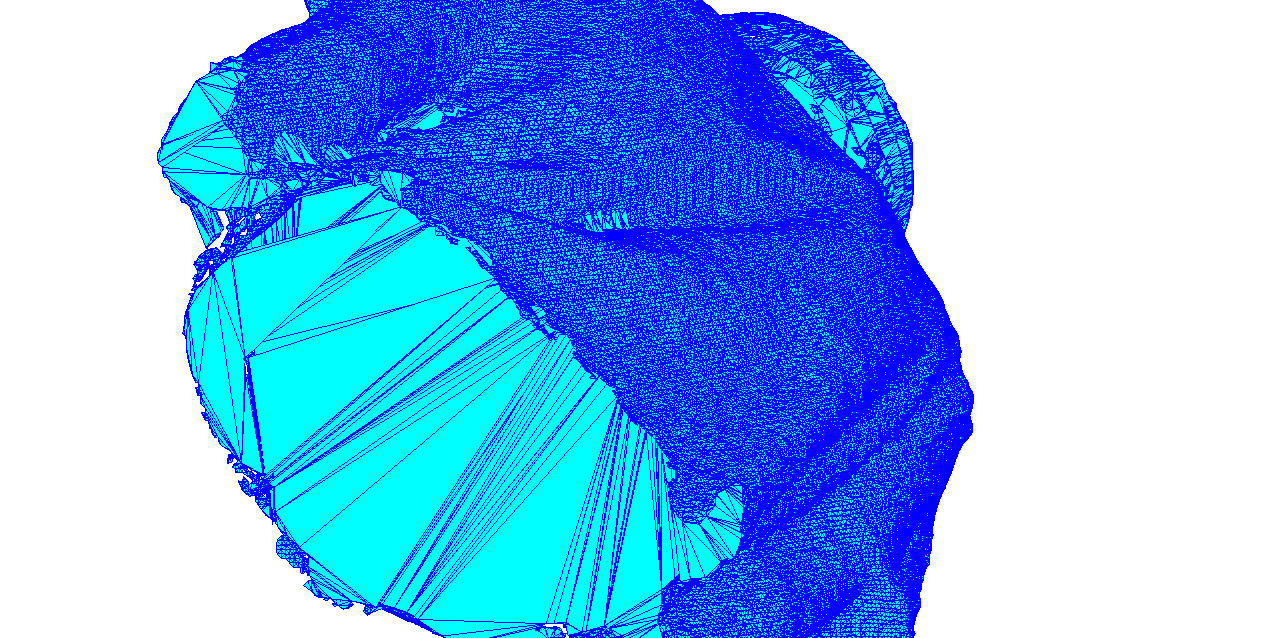
\includegraphics[width=0.49\textwidth]{figures/3dMesh_sundin_zoom_bot.png}
    \caption{Printable triangular mesh, bot view}
    \label{fig:sundin-top-zoom}
\end{figure}